\documentclass[border=3pt]{standalone}
% Preâmbulo compartilhado pelos diagramas TikZ da aula 6 de IHC (Necessidades e Requisitos)
\usepackage[T1]{fontenc}
\usepackage[utf8]{inputenc}
\usepackage{lmodern}
\usepackage{amsmath}
\usepackage{xcolor}
\usepackage{tikz}
\usetikzlibrary{arrows.meta,angles,quotes,decorations.pathmorphing,calc,
                positioning,shapes.geometric,shapes.misc,backgrounds,fit,
                math}

% Paleta (mesma dos SVGs originais)
% Paleta da disciplina de IHC: acento roxo (#755099), da capa do livro.
% (o nome "dblue" é mantido para não alterar todos os diagramas)
\definecolor{dblue}{HTML}{755099}
\definecolor{dorange}{HTML}{B3541E}
\definecolor{dgreen}{HTML}{4A7C59}
\definecolor{dred}{HTML}{9C4B4B}
\definecolor{dcream}{HTML}{F4F1EA}
\definecolor{dshade}{HTML}{DDD7C9}

% Função gaussiana (não normalizada por padrão de escala visual)
\pgfmathdeclarefunction{gauss}{3}{%
  \pgfmathparse{1/(#3*sqrt(2*pi))*exp(-((#1-#2)^2)/(2*#3^2))}%
}

% Estilos comuns (prefixo d... para não colidir com chaves internas do pgf)
\tikzset{
  >={Stealth[length=2mm]},
  dguide/.style={gray!55, dashed, line width=0.4pt},
  daxis/.style={gray!60, line width=0.7pt, ->},
  dbody/.style={fill=black!3, draw=black!80, line width=1pt},
  dacc/.style={draw=dblue, line width=1pt},
  dlbl/.style={black!55, font=\small},
  dsub/.style={black!45, font=\footnotesize},
  dstate/.style={circle, draw=black!80, fill=dcream, line width=1pt,
                 minimum size=17mm, font=\large, inner sep=1pt},
  dobs/.style={circle, draw=black!80, fill=dshade, line width=1pt,
               minimum size=14mm, font=\large, inner sep=1pt},
  dbox/.style={rounded corners=2pt, draw=black!80, fill=dcream, line width=1pt,
               align=center, inner sep=6pt},
  dop/.style={circle, draw=black!80, fill=white, line width=1pt,
              minimum size=6mm, inner sep=0pt, font=\small},
  dtrans/.style={->, dblue, line width=1pt},
  dmeas/.style={->, dorange, line width=1pt},
  dcurve/.style={line width=1pt, dblue},
  dcurveb/.style={line width=1.4pt, dorange},
}

\begin{document}
\hyphenpenalty=10000 \exhyphenpenalty=10000 \tolerance=9999 \emergencystretch=3em
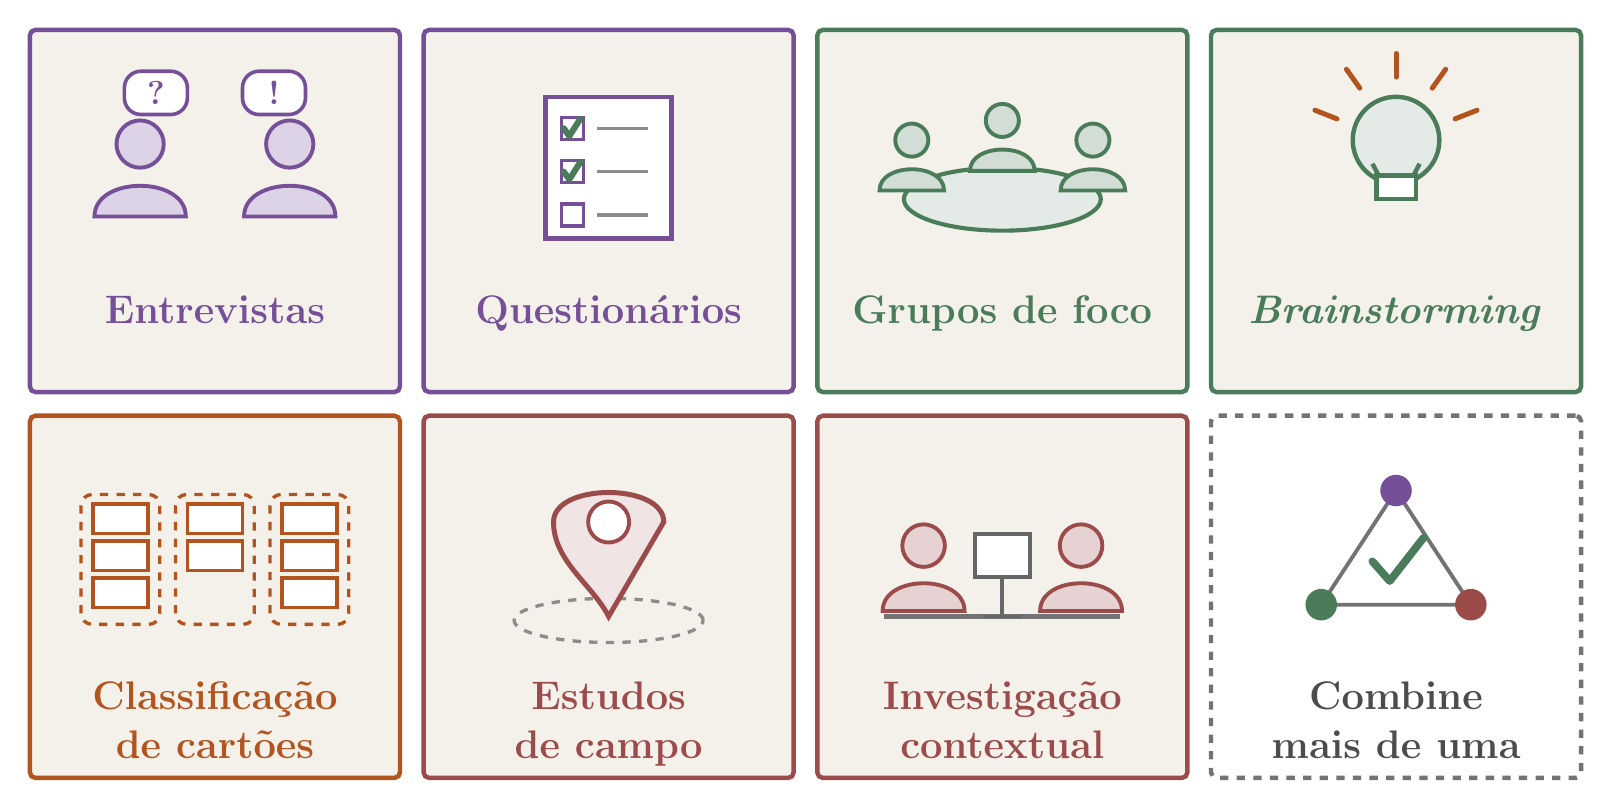
\begin{tikzpicture}[x=1cm,y=1cm]
\node[dbox, draw=dblue, line width=1.6pt, minimum width=4.7cm, minimum height=4.6cm] at (2.35,7.20) {};
\node[font=\Large\bfseries, dblue, text width=4.3cm, align=center, anchor=north] at (2.35,6.25) {Entrevistas};
\fill[dblue!25!white, draw=dblue, line width=1.4pt] (1.40,8.05) circle (0.30);
\fill[dblue!25!white, draw=dblue, line width=1.4pt] (0.82,7.13) .. controls (0.82,7.65) and (1.98,7.65) .. (1.98,7.13) -- cycle;
\fill[dblue!25!white, draw=dblue, line width=1.4pt] (3.30,8.05) circle (0.30);
\fill[dblue!25!white, draw=dblue, line width=1.4pt] (2.72,7.13) .. controls (2.72,7.65) and (3.88,7.65) .. (3.88,7.13) -- cycle;
\node[draw=dblue, fill=white, line width=1.3pt, rounded corners=6pt, minimum width=0.8cm, minimum height=0.55cm, font=\large\bfseries, text=dblue] at (1.60,8.70) {?};
\node[draw=dblue, fill=white, line width=1.3pt, rounded corners=6pt, minimum width=0.8cm, minimum height=0.55cm, font=\large\bfseries, text=dblue] at (3.10,8.70) {!};
\node[dbox, draw=dblue, line width=1.6pt, minimum width=4.7cm, minimum height=4.6cm] at (7.35,7.20) {};
\node[font=\Large\bfseries, dblue, text width=4.3cm, align=center, anchor=north] at (7.35,6.25) {Questionários};
\draw[dblue, fill=white, line width=1.6pt] (6.55,6.85) rectangle (8.15,8.65);
\draw[dblue, line width=1.2pt] (6.75,8.11) rectangle ++(0.28,0.28);
\draw[black!45, line width=1.3pt] (7.20,8.25) -- ++(0.65,0);
\draw[dgreen, line width=2.2pt, line cap=round, line join=round] (6.78,8.25) -- (6.85,8.15) -- (6.99,8.37);
\draw[dblue, line width=1.2pt] (6.75,7.56) rectangle ++(0.28,0.28);
\draw[black!45, line width=1.3pt] (7.20,7.70) -- ++(0.65,0);
\draw[dgreen, line width=2.2pt, line cap=round, line join=round] (6.78,7.70) -- (6.85,7.60) -- (6.99,7.82);
\draw[dblue, line width=1.2pt] (6.75,7.01) rectangle ++(0.28,0.28);
\draw[black!45, line width=1.3pt] (7.20,7.15) -- ++(0.65,0);
\node[dbox, draw=dgreen, line width=1.6pt, minimum width=4.7cm, minimum height=4.6cm] at (12.35,7.20) {};
\node[font=\Large\bfseries, dgreen, text width=4.3cm, align=center, anchor=north] at (12.35,6.25) {Grupos de foco};
\draw[dgreen, fill=dgreen!15!white, line width=1.5pt] (12.35,7.35) ellipse (1.25 and 0.4);
\fill[dgreen!25!white, draw=dgreen, line width=1.4pt] (11.20,8.10) circle (0.21);
\fill[dgreen!25!white, draw=dgreen, line width=1.4pt] (10.79,7.46) .. controls (10.79,7.82) and (11.61,7.82) .. (11.61,7.46) -- cycle;
\fill[dgreen!25!white, draw=dgreen, line width=1.4pt] (12.35,8.35) circle (0.21);
\fill[dgreen!25!white, draw=dgreen, line width=1.4pt] (11.94,7.71) .. controls (11.94,8.07) and (12.76,8.07) .. (12.76,7.71) -- cycle;
\fill[dgreen!25!white, draw=dgreen, line width=1.4pt] (13.50,8.10) circle (0.21);
\fill[dgreen!25!white, draw=dgreen, line width=1.4pt] (13.09,7.46) .. controls (13.09,7.82) and (13.91,7.82) .. (13.91,7.46) -- cycle;
\node[dbox, draw=dgreen, line width=1.6pt, minimum width=4.7cm, minimum height=4.6cm] at (17.35,7.20) {};
\node[font=\Large\bfseries, dgreen, text width=4.3cm, align=center, anchor=north] at (17.35,6.25) {\emph{Brainstorming}};
\draw[dgreen, fill=dgreen!15!white, line width=1.6pt] (17.35,8.10) circle (0.55);
\draw[dgreen, line width=1.6pt, fill=white] (17.10,7.35) rectangle (17.60,7.65);
\draw[dgreen, line width=1.6pt] (17.13,7.65) -- (17.05,7.80) (17.57,7.65) -- (17.65,7.80);
\draw[dorange, line width=1.8pt, line cap=round] (18.10,8.37) -- (18.38,8.48);
\draw[dorange, line width=1.8pt, line cap=round] (17.81,8.76) -- (17.98,9.00);
\draw[dorange, line width=1.8pt, line cap=round] (17.35,8.90) -- (17.35,9.20);
\draw[dorange, line width=1.8pt, line cap=round] (16.89,8.76) -- (16.72,9.00);
\draw[dorange, line width=1.8pt, line cap=round] (16.60,8.37) -- (16.32,8.48);
\node[dbox, draw=dorange, line width=1.6pt, minimum width=4.7cm, minimum height=4.6cm] at (2.35,2.30) {};
\node[font=\Large\bfseries, dorange, text width=4.3cm, align=center, anchor=north] at (2.35,1.35) {Classificação de cartões};
\draw[dorange, dashed, line width=1.2pt, rounded corners=4pt] (0.65,1.95) rectangle (1.65,3.60);
\draw[dorange, fill=white, line width=1.2pt] (0.80,3.10) rectangle ++(0.7,0.38);
\draw[dorange, fill=white, line width=1.2pt] (0.80,2.63) rectangle ++(0.7,0.38);
\draw[dorange, fill=white, line width=1.2pt] (0.80,2.16) rectangle ++(0.7,0.38);
\draw[dorange, dashed, line width=1.2pt, rounded corners=4pt] (1.85,1.95) rectangle (2.85,3.60);
\draw[dorange, fill=white, line width=1.2pt] (2.00,3.10) rectangle ++(0.7,0.38);
\draw[dorange, fill=white, line width=1.2pt] (2.00,2.63) rectangle ++(0.7,0.38);
\draw[dorange, dashed, line width=1.2pt, rounded corners=4pt] (3.05,1.95) rectangle (4.05,3.60);
\draw[dorange, fill=white, line width=1.2pt] (3.20,3.10) rectangle ++(0.7,0.38);
\draw[dorange, fill=white, line width=1.2pt] (3.20,2.63) rectangle ++(0.7,0.38);
\draw[dorange, fill=white, line width=1.2pt] (3.20,2.16) rectangle ++(0.7,0.38);
\node[dbox, draw=dred, line width=1.6pt, minimum width=4.7cm, minimum height=4.6cm] at (7.35,2.30) {};
\node[font=\Large\bfseries, dred, text width=4.3cm, align=center, anchor=north] at (7.35,1.35) {Estudos de campo};
\draw[black!45, dashed, line width=1.2pt] (7.35,2.00) ellipse (1.2 and 0.28);
\draw[dred, fill=dred!15!white, line width=1.8pt] (7.35,2.05) .. controls (7.15,2.45) and (6.65,2.75) .. (6.65,3.25) .. controls (6.65,3.75) and (8.05,3.75) .. (8.05,3.25) -- cycle;
\fill[white, draw=dred, line width=1.4pt] (7.35,3.25) circle (0.26);
\node[dbox, draw=dred, line width=1.6pt, minimum width=4.7cm, minimum height=4.6cm] at (12.35,2.30) {};
\node[font=\Large\bfseries, dred, text width=4.3cm, align=center, anchor=north] at (12.35,1.35) {Investigação contextual};
\draw[black!55, line width=1.6pt] (10.85,2.05) -- (13.85,2.05);
\fill[dred!25!white, draw=dred, line width=1.4pt] (11.35,2.95) circle (0.27);
\fill[dred!25!white, draw=dred, line width=1.4pt] (10.83,2.12) .. controls (10.83,2.59) and (11.87,2.59) .. (11.87,2.12) -- cycle;
\fill[dred!25!white, draw=dred, line width=1.4pt] (13.35,2.95) circle (0.27);
\fill[dred!25!white, draw=dred, line width=1.4pt] (12.83,2.12) .. controls (12.83,2.59) and (13.87,2.59) .. (13.87,2.12) -- cycle;
\draw[black!60, fill=white, line width=1.4pt] (12.00,2.55) rectangle (12.70,3.10);
\draw[black!60, line width=1.4pt] (12.35,2.55) -- (12.35,2.05) (12.10,2.05) -- (12.60,2.05);
\node[dbox, draw=black!55, dashed, fill=white, line width=1.6pt, minimum width=4.7cm, minimum height=4.6cm] at (17.35,2.30) {};
\node[font=\Large\bfseries, black!70, text width=4.3cm, align=center, anchor=north] at (17.35,1.35) {Combine mais de uma};
\draw[black!55, line width=1.4pt] (17.35,3.65) -- (16.40,2.20) -- (18.30,2.20) -- cycle;
\fill[dblue] (17.35,3.65) circle (0.2);
\fill[dgreen] (16.40,2.20) circle (0.2);
\fill[dred] (18.30,2.20) circle (0.2);
\draw[dgreen, line width=2.8pt, line cap=round, line join=round] (17.05,2.75) -- (17.27,2.50) -- (17.70,3.05);
\end{tikzpicture}
\end{document}
